\documentclass[%
% jmp,
% bmf,
% sd,
% rsi,
twocolumn,
amsmath,amssymb,
groupedaddress,
% preprint,%
reprint,%
% author-year,%
% author-numerical,%
% Conference Proceedings
]{revtex4-2}

\usepackage{bm}
\usepackage{listings}
\lstset{language=Python,keywordstyle={\bfseries \color{blue}}}

\usepackage{tikz}
\usetikzlibrary{arrows.meta,
	chains,
	matrix,
  decorations,
	positioning,
  calc,
  decorations.pathmorphing,
  shapes.geometric}

\renewcommand{\d}{{\rm d}}
\newcommand{\w}{\omega}
\newcommand{\wti}{\widetilde}
\newcommand{\ti}{\tilde}
\newcommand{\B}{\mathrm{B}}
\newcommand{\D}{\mathrm{D}}
\newcommand{\Bs}{\mathrm{Bose}}
\newcommand{\s}{\mathrm{S}}
\newcommand{\tT}{\mathrm{T}}
\newcommand{\tB}{\mathrm{B}}
\newcommand{\tW}{\mathrm{W}}
\newcommand{\tS}{\mathrm{S}}
\newcommand{\st}{\mathrm{st}}
\newcommand{\te}{\mathrm{e}}
\newcommand{\tg}{\mathrm{g}}
\newcommand{\T}{\mathrm{T}}
\newcommand{\tR}{\mathrm{R}}
\newcommand{\tL}{\mathrm{L}}
\newcommand{\tM}{\mathrm{M}}
\newcommand{\tc}{\mathrm{c}}
\newcommand{\app}{\mathrm{app}}
\newcommand{\tot}{\mathrm{tot}}
\newcommand{\SB}{\mathrm{SB}}
\newcommand{\tr}{\mathrm{tr}}
\newcommand{\Tr}{\mathrm{Tr}}
\newcommand{\dg}{\dagger}
\newcommand{\la}{\langle}
\newcommand{\ra}{\rangle}
\renewcommand{\>}{\rangle}
\newcommand{\<}{\langle}
\newcommand{\lla}{\langle\langle}
\newcommand{\rra}{\rangle\rangle}
\newcommand{\La}{\big\la}
\newcommand{\Ra}{\big\ra}
\newcommand{\BO}{\mathrm{BO}}
\newcommand{\cm}{\mathrm{cm}^{\mathrm{-1}}}
% \newcommand{\Ref}[1]{Ref.\,\onlinecite{#1}}
\newcommand{\Sec}[1]{Sec.\,\ref{#1}}
\newcommand{\nl}{\nonumber \\}
\newcommand{\be}{\begin{equation}}
\newcommand{\ee}{\end{equation}}
\newcommand{\bsube}{\begin{subequations}}
\newcommand{\esube}{\end{subequations}}
\newcommand{\Eq}[1]{Equation \,(\ref{#1})}
\newcommand{\eq}[1]{Eq.\,(\ref{#1})}
\newcommand{\Eqs}[1]{Equations .\,(\ref{#1})}
\newcommand{\eqs}[1]{Equations .\,(\ref{#1})}
\newcommand{\Fig}[1]{Fig.\,\ref{#1}}
\newcommand{\Tab}[1]{Table \ref{#1}}
\newcommand{\obarplus}{\mbox{\tiny$\oplus$}}
\newcommand{\obarminus}{\mbox{\tiny$\ominus$}}
\newcommand{\greater}{\mathrm{$>$}}
\newcommand{\lesser}{\mathrm{$<$}}
\newcommand{\lgter}{\mathrm{$\lessgtr$}}
\newcommand{\gler}{\mathrm{$\gtrless$}}
\newcommand{\WF}{\mathrm{WF}}
\newcommand{\KS}{\mathrm{KS}}
\newcommand{\XC}{\mathrm{XC}}
\renewcommand{\L}{\mathrm{L}}
\renewcommand{\P}{\mathrm{P}}
\newcommand{\brm}[1]{\bm{\mathrm{#1}}}
\newcommand{\ext}{\mathrm{ext}}

\newcommand{\blue}[1]{\textcolor{blue}{#1}}
\newcommand{\red}[1]{\textcolor{red}{#1}}
\begin{document}


\title{Approaching the precision energy surface in the local density approximation level density functional theory}
\author{XX}

\date{\today}

\begin{abstract}
    %%
    {
        TODO
    }
\end{abstract}

\maketitle

\section{Introduction}
In this article, we combine the machine learning (ML) method and density functional theory (DFT) to predict the properties of the molecules.
% 
By predicting both the potential and the energy from the electron density of the molecule using the ML method, we can calculate the properties of the molecule, such as the energy, the bond length, and the dipole moment.
% 
The ML method is based on the well-developed UNET architecture, which is a convolutional neural network (CNN) for fast and precise segmentation of images \cite{Ronneberger2015}.
% 
The target potential and the target energy are obtained from the inverse DFT calculation, in this article, we use the modified Ryabinkin-Kohut-Staroverov method.

\section{Methods}
The density functional theory has dominated quantum chemistry calculation in the last few decades, especially in the large molecular system.
% 
One of the standard methods is the Kohn-Sham (KS) DFT, which is based on the Hohenberg-Kohn theorem and the Kohn-Sham equation.
% 
The KS DFT can be written as
\begin{subequations}
    \label{eq:ksdft}
    \begin{align}
        E[\rho(\brm{r})] = T_{\tS}[\rho(\brm{r})] + E_{\textrm{J}}[\rho(\brm{r})] + & E_{\XC}[\rho(\brm{r})] + E_{\ext}[\rho(\brm{r})], \\
        \int d \brm{r} \rho(\brm{r})                                                & = N.
    \end{align}
\end{subequations}
where
The $N$ is the total number of electrons in the system, $E_{\XC}[\rho(\brm{r})]$ is the exchange-correlation energy functional which has many forms and
\begin{subequations}
    \begin{align}
        T_{\tS}[\rho(\brm{r})]        & = -\frac{1}{2} \nabla^2 \rho(\brm{r}),                                                                                  \\
        E_{\textrm{J}}[\rho(\brm{r})] & = \frac{1}{2} \int d \brm{r}_{i} d \brm{r}_{j} \frac{\rho(\brm{r}_{i}) \rho(\brm{r}_{j})}{|\brm{r}_{i} - \brm{r}_{j}|}, \\
        E_{\ext}[\rho(\brm{r})]       & = \int d \brm{r} \rho(\brm{r}) V_{\ext}(\brm{r}).
    \end{align}
\end{subequations}
Here, the $V_{\ext}(\brm{r})$ is the external potential. For example, the nuclear potential caused by ions with Z number of charge at position $R$, $V_{\ext}(\brm{r}) = \int d \brm{r} \frac{Z \rho(\brm{r})}{|\brm{r}-R|}$.

Solve \Eq{eq:ksdft} directly caused the high computational cost, one of the common methods is to use the finite basis set.
% 
The finite basis set starts with expanding the molecular orbital as the linear combination of the atom orbital,
\begin{equation}
    \phi^{\sigma}_i(\brm{r}) = \sum_{\mu} C^{\sigma}_{\mu i} \chi_{\mu}(\brm{r}),
\end{equation}
here we use $i$ to index the molecular orbital $\sigma$ to index the spin and $\mu$ to index the basis set.
% 
The density $\rho(\brm{r}_{i})$ can be rewritten as
\begin{equation}
    \begin{aligned}
        \rho^{\sigma}(\brm{r}) = \sum_{\mu \nu} P^{\sigma}_{\mu \nu} \chi_{\mu}(\brm{r}) \chi_{\nu}(\brm{r}),
    \end{aligned}
\end{equation}
where $P^{\sigma}_{\mu \nu} = \sum_{i}^{N_{\sigma}} C_{\mu i} C_{\nu i}$.

The energy functional can be written as
\begin{align}
      & E[\rho^{{\sigma}}(\brm{r})] = E[P^{\sigma}_{\mu \nu}] \nl
    = & \sum_{\mu \nu} P^{\sigma}_{\mu \nu} H^{\sigma}_{\mu \nu} + \frac{1}{2} \sum_{ijkl} P^{\sigma}_{ij} J^{\sigma}_{ijkl} P^{\sigma}_{kl}  \nl
      & + \sum_{\mu \nu}  E_{\XC}[P^{\sigma}_{\mu \nu}] P^{\sigma}_{\mu \nu}.
\end{align}

\section{Results}
We use carbon-hydrogen molecules with difference bond lengths in the g2/97 dataset as the training set, and the test set is the Pentane.
%
The performance of the ML model is shown below,
\begin{table}[h]
    \centering
    \begin{tabular}{c|c|c}
        \hline
        Molecule     & Energy (mH) & density (me) \\
        \hline
        training set & 18.02       & 71.45        \\
        test set     & 89.47       & 231.23       \\
        \hline
    \end{tabular}
    \caption{The performance of the ML model}
\end{table}

\begin{figure*}
    \centering
    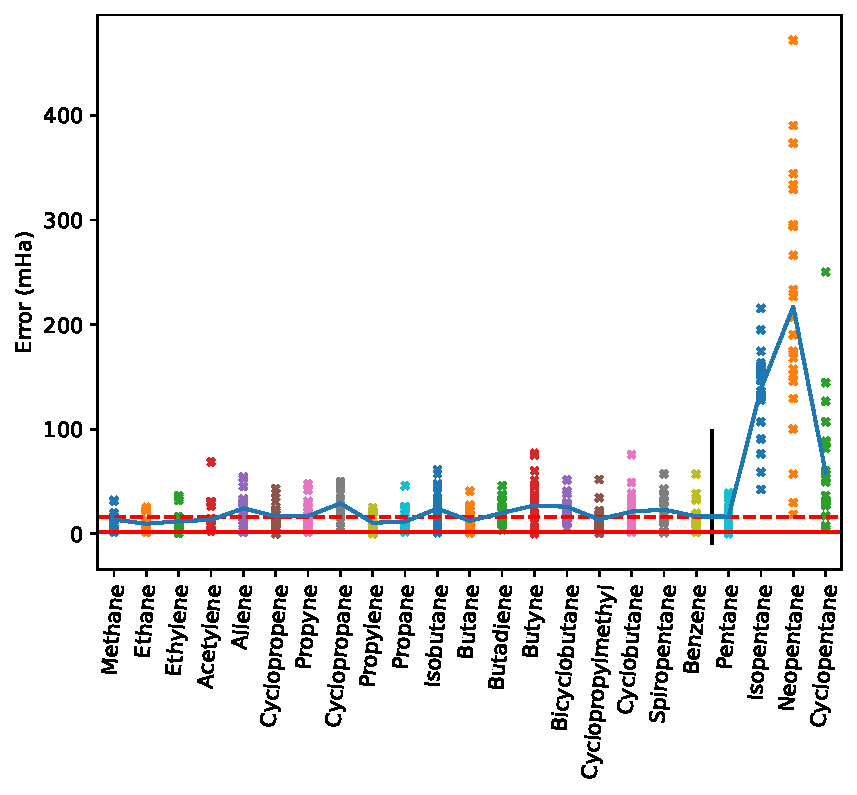
\includegraphics[width=0.95\textwidth]{figures/energy.pdf}
    \caption{The energy of the Pentane molecule}
\end{figure*}
% Then the self-consistent field (SCF) can be written as
% \begin{equation}
%     F = H^{\sigma} + J + V = \epsilon^{\sigma}_{i} C S^{\sigma} C^{-1},
% \end{equation}
\end{document}
